\chapter{连续系统}
\label{ch:7}

\section*{7.1　弦}

弦的两端被拉伸固定于 $x_1$ 和 $x_2$ 两点之间。弦中的张力为 $\tau$。弦的单位长度质量为 $\lambda$。你可以想象弦被拨动，激起了一列波。

\begin{figure}[h]
\centering
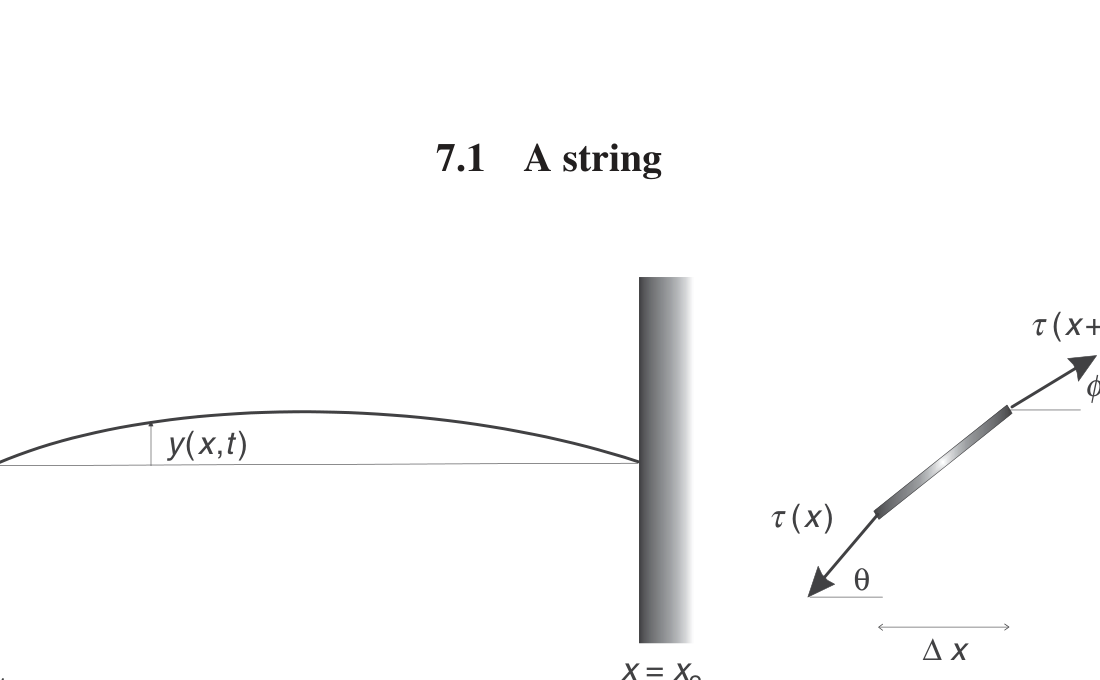
\includegraphics[width=0.55\linewidth]{../Figures/fig_7_1.png}
\caption{图 7.1　左：一根振动的弦。右：位于 $x$ 处的弦元，受到张力 $\tau(x + dx)$ 与 $\tau(x)$ 的作用。}
\end{figure}

在时刻 $t$，弦上位置 $x$ 处的位移为 $y = y(x, t)$。在用变分的观点处理这个问题之前，让我们先用牛顿第二定律简要地过一遍波动方程的基本推导。考虑长度为 $dx$ 的一个弦元。它的质量为 $\lambda\,dx$。作用在它上面的力是两端所受的张力，即 $\tau(x)$ 和 $\tau(x + dx)$，如图所示。

图是高度夸张的，弦其实非常贴近水平的 $x$ 轴。因此
$$
\sin\theta \simeq \tan\theta = \lim_{\Delta x \to 0}\frac{\Delta y}{\Delta x} = \frac{\partial y(x, t)}{\partial x}.
$$
由 $ma = F$ 我们有
$$
\lambda(x)\,dx\,\frac{\partial^2 y}{\partial t^2} = \tau(x + dx)\sin\phi - \tau(x)\sin\theta,
$$
即
$$
= \tau(x + dx)\frac{\partial y(x + dx, t)}{\partial x} - \tau(x)\frac{\partial y(x, t)}{\partial x},
$$
展开第一项
$$
= \left[\tau(x)\frac{\partial y(x, t)}{\partial x} + dx\,\frac{\partial}{\partial x}\left(\tau(x)\frac{\partial y(x, t)}{\partial x}\right) + \cdots\right] - \tau(x)\frac{\partial y(x, t)}{\partial x},
$$
其中我们把第一项作了泰勒级数展开。于是
$$
\lambda(x)\frac{\partial^2 y}{\partial t^2} = \frac{\partial}{\partial x}\left[\tau(x)\frac{\partial y}{\partial x}\right]. \eqno\hbox{(7.1)}
$$

为简单起见，我们假设 $\lambda$ 和 $\tau$ 都不是 $x$ 的函数。于是
$$
\frac{\partial^2 y}{\partial t^2} = \frac{\tau}{\lambda}\frac{\partial^2 y}{\partial x^2},
$$
这就是波动方程。波的传播速度为 $\sqrt{\tau/\lambda}$。

由此可见，$F = ma$ 把我们引向波动方程。但我们感兴趣的是用拉格朗日方法得到这一结果。我将通过引入单位长度的拉格朗日量，即拉格朗日密度（记为 $\mathcal{L}$），来为连续弦写出合适的拉格朗日量。系统的拉格朗日量为
$$
L = \int_{x_1}^{x_2}\mathcal{L}\,dx.
$$
不难看出，弦元的动能密度可以表示为 $\frac{1}{2}\lambda\,dx\,\dot{y}^2$，其中 $\lambda\,dx$ 是长度为 $dx$ 的弦元的质量，$\dot{y}$ 是它的竖直速度。势能应该取什么形式则不那么明显。但请注意，力 $\dfrac{\partial}{\partial x}\left[\tau(x)\dfrac{\partial y}{\partial x}\right]dx$ 通过 $F = -\partial V/\partial x$ 与势能相联系，所以势能可以写成 $\frac{1}{2}\tau y'^2\,dx$，其中 $y' = \partial y/\partial x$。于是系统的拉格朗日量可以写成
$$
L = \int_{x_1}^{x_2}\mathcal{L}\,dx = \int_{x_1}^{x_2}\left[\frac{1}{2}\lambda(x)\dot{y}^2 - \frac{1}{2}\tau(x)y'^2\right]dx.
$$
如果作合理的假设，认为质量密度 $\lambda$ 和张力 $\tau$ 均为常数，则得到
$$
L = \frac{\lambda}{2}\int_{x_1}^{x_2}\dot{y}^2\,dx - \frac{\tau}{2}\int_{x_1}^{x_2}y'^2\,dx,
$$
于是该系统的拉格朗日密度为
$$
\mathcal{L} = \frac{\lambda}{2}\dot{y}^2 - \frac{\tau}{2}y'^2.
$$
这常常写成更明确的形式：
$$
\mathcal{L} = \frac{\lambda}{2}\left(\frac{\partial y}{\partial t}\right)^2 - \frac{\tau}{2}\left(\frac{\partial y}{\partial x}\right)^2. \eqno\hbox{(7.2)}
$$

\begin{exercise}
证明：若势能由 $\frac{1}{2}\tau y'^2$ 给出，则作用力由方程（7.1）右端的表达式给出。
\end{exercise}

\begin{exercise}
考虑弦中的一列行波，其通常表述为 $y(x, t) = A\cos(kx - \omega t)$。$k$、$\omega$ 与 $\lambda$、$\tau$ 之间有何关系？
\end{exercise}

下面让我们确定该系统拉格朗日方程的合适形式。回到基本原理，我们回想起拉格朗日方程是哈密顿原理的推论，哈密顿原理我们已表述为
$$
\delta\int_{t_1}^{t_2}L\,dt = 0.
$$
也就是说，端点 $t_1$ 与 $t_2$ 之间作用量的变分为零。但对于我们这一分布的一维系统，拉格朗日量可能沿弦的位置而变化。（显然，弦上质点的速度既依赖于 $t$，也依赖于 $x$。）假定拉格朗日量是分布式的，系统的总拉格朗日量为
$$
L = \int_{x_1}^{x_2}\mathcal{L}\,dx,
$$
哈密顿原理于是变为
$$
\delta\int_{t_1}^{t_2}\int_{x_1}^{x_2}\mathcal{L}\,dx\,dt = 0.
$$
让我们考察拉格朗日密度的函数依赖关系。它将显式地依赖于位置和时间（$x$ 与 $t$），因为它们是自变量。但我们预期它将隐式地依赖于位移 $y$、竖直方向的速度 $\dot{y} = \partial y/\partial t$ 以及"伸长" $y' = \partial y/\partial x$。即
$$
\mathcal{L} = \mathcal{L}(y, \dot{y}, y'; x, t).
$$
注意，自变量 $x$ 和 $t$ 正是哈密顿原理中的积分变量。某一特定位置和时刻的拉格朗日密度一般将依赖于 $y$、$\dot{y}$ 和 $y'$。我们可以把 $y$ 看作确定系统构形的广义坐标。它将在哈密顿原理中被变分。它在端点处的变分必须为零。但现在我们有两组端点，既涉及位置也涉及时间。注意，我们并不是说 $y$ 本身在边界上为零，而只是说它在边界处的变分为零。即
$$
\delta(y(t_1)) = \delta(y(t_2)) = 0,
$$
以及
$$
\delta(y(x_1)) = \delta(y(x_2)) = 0.
$$
这仅仅意味着我们要求所有的"路径"$y(x, t)$ 都从 $(x_1, t_1)$ 出发，并在 $(x_2, t_2)$ 终止。例如，在初始时刻，变分后的弦构形上的所有位置都对应于实际的初始构形；而在任何时刻，变分后的弦构形的端点都对应于实际的构形（碰巧是 $y(x_1, t) = 0$ 和 $y(x_2, t) = 0$）。

哈密顿原理为
$$
0 = \delta\int_{t_1}^{t_2}L\,dt = \delta\int_{t_1}^{t_2}dt\int_{x_1}^{x_2}dx\,\mathcal{L}(y, y', \dot{y}; x, t)
$$
$$
= \int_{t_1}^{t_2}dt\int_{x_1}^{x_2}dx\left[\frac{\partial\mathcal{L}}{\partial y}\delta y + \frac{\partial\mathcal{L}}{\partial y'}\delta y' + \frac{\partial\mathcal{L}}{\partial\dot{y}}\delta\dot{y}\right]. \eqno\hbox{(7.3)}
$$
注意
$$
\delta y' = \delta\left(\frac{\partial y}{\partial x}\right) = \frac{\partial}{\partial x}\delta y,
$$
其中 $t$ 保持固定，
以及
$$
\delta\dot{y} = \delta\left(\frac{\partial y}{\partial t}\right) = \frac{\partial}{\partial t}\delta y,
$$
其中 $x$ 保持固定。

考虑方程（7.3）中的第一项，并牢记 $y$（以及 $\dot{y}$）是沿变分路径上的值（例如表示为方程（2.5）中的 $Y$）：
$$
\int_{t_1}^{t_2}dt\int_{x_1}^{x_2}dx\,\frac{\partial\mathcal{L}}{\partial\dot{y}}\delta\dot{y}
= \int_{t_1}^{t_2}dt\int_{x_1}^{x_2}dx\,\frac{\partial\mathcal{L}}{\partial\dot{y}}\frac{\partial\dot{y}}{\partial\epsilon}\delta\epsilon
$$
$$
= \int_{x_1}^{x_2}dx\int_{t_1}^{t_2}dt\,\frac{\partial\mathcal{L}}{\partial\dot{y}}\frac{\partial}{\partial\epsilon}\left(\frac{\partial y}{\partial t}\right)\delta\epsilon
$$
$$
= \int_{x_1}^{x_2}dx\int_{t_1}^{t_2}dt\,\frac{\partial\mathcal{L}}{\partial\dot{y}}\frac{\partial}{\partial t}\left(\frac{\partial y}{\partial\epsilon}\right)\delta\epsilon.
$$
分部积分：
$$
\int_{t_1}^{t_2}dt\int_{x_1}^{x_2}dx\,\frac{\partial\mathcal{L}}{\partial\dot{y}}\delta\dot{y}
= \int_{x_1}^{x_2}dx\,\delta\epsilon\left[\frac{\partial\mathcal{L}}{\partial\dot{y}}\frac{\partial y}{\partial\epsilon}\right]_{t_1}^{t_2} - \int_{t_1}^{t_2}dt\,\frac{\partial}{\partial t}\left(\frac{\partial\mathcal{L}}{\partial\dot{y}}\frac{\partial y}{\partial\epsilon}\right)\delta\epsilon
$$
$$
= \int_{x_1}^{x_2}dx\left[0 - \int_{t_1}^{t_2}dt\,\frac{\partial}{\partial t}\left(\frac{\partial\mathcal{L}}{\partial\dot{y}}\right)\delta y\right]
$$
$$
= -\int_{t_1}^{t_2}dt\int_{x_1}^{x_2}dx\,\frac{\partial}{\partial t}\left(\frac{\partial\mathcal{L}}{\partial\dot{y}}\right)\delta y.
$$
类似地，我们可以把方程（7.3）中的第二项分部积分，得到
$$
\int_{t_1}^{t_2}dt\int_{x_1}^{x_2}dx\,\frac{\partial\mathcal{L}}{\partial y'}\delta y' = \int_{t_1}^{t_2}\int_{x_1}^{x_2}dt\,dx\,(-1)\frac{\partial}{\partial x}\left(\frac{\partial\mathcal{L}}{\partial y'}\right),
$$
其中我们利用了变分在端点处消失这一事实。

总而言之，我们认识到哈密顿原理可以表示为
$$
0 = \int_{t_1}^{t_2}dt\int_{x_1}^{x_2}dx\left[\frac{\partial\mathcal{L}}{\partial y} - \frac{\partial}{\partial x}\left(\frac{\partial\mathcal{L}}{\partial y'}\right) - \frac{\partial}{\partial t}\left(\frac{\partial\mathcal{L}}{\partial\dot{y}}\right)\right]\delta y.
$$
与往常一样，哈密顿原理导出了拉格朗日方程。在上面的方程中我们注意到，变分 $\delta y$ 是任意的，所以括号中的项必须为零。于是我们得到一维连续系统拉格朗日方程的一般形式：
$$
\frac{\partial}{\partial t}\left(\frac{\partial\mathcal{L}}{\partial\dot{y}}\right) + \frac{\partial}{\partial x}\left(\frac{\partial\mathcal{L}}{\partial y'}\right) - \frac{\partial\mathcal{L}}{\partial y} = 0. \eqno\hbox{(7.4)}
$$
我们可以把它写成更明确但也更复杂的形式：
$$
\frac{\partial}{\partial t}\left(\frac{\partial\mathcal{L}}{\partial(\partial y/\partial t)}\right) + \frac{\partial}{\partial x}\left(\frac{\partial\mathcal{L}}{\partial(\partial y/\partial x)}\right) - \frac{\partial\mathcal{L}}{\partial y} = 0.
$$
作为一个简单的应用，让我们把这一形式的拉格朗日方程应用于弦的拉格朗日密度：
$$
\mathcal{L} = \frac{\lambda}{2}\left(\frac{\partial y}{\partial t}\right)^2 - \frac{\tau}{2}\left(\frac{\partial y}{\partial x}\right)^2.
$$
我们看出
$$
\frac{\partial\mathcal{L}}{\partial\dot{y}} = \lambda\dot{y}, \qquad \frac{\partial\mathcal{L}}{\partial y'} = -\tau y', \qquad \frac{\partial\mathcal{L}}{\partial y} = 0,
$$
于是方程（7.4）给出
$$
\frac{\partial}{\partial t}(\lambda\dot{y}) + \frac{\partial}{\partial x}(-\tau y') = 0,
$$
即
$$
\lambda\ddot{y} - \tau y'' = 0.
$$
也就是说
$$
\frac{\partial^2 y}{\partial t^2} = \frac{\tau}{\lambda}\frac{\partial^2 y}{\partial x^2},
$$
这就是波动方程。

\section*{7.2　推广到三维}

我们曾把一维系统的拉格朗日密度表示为
$$
\mathcal{L} = \mathcal{L}(y, \dot{y}, y'; x, t),
$$
或
$$
\mathcal{L} = \mathcal{L}\left(y, \frac{\partial y}{\partial t}, \frac{\partial y}{\partial x}; x, t\right).
$$
推广到三维，令系统的构形由标量坐标 $w = w(x, y, z, t)$ 确定。我们把 $y$ 换成 $w$，把 $\dot{y}$ 换成 $\dot{w} = \partial w/\partial t$。这是直截了当的。但现在我们需要把 $y'$ 换成 $w$ 对 $x, y, z$ 的导数，具体地说，换成 $\partial w/\partial x$、$\partial w/\partial y$、$\partial w/\partial z$。回忆矢量恒等式 $\nabla w = \hat{x}\frac{\partial w}{\partial x} + \hat{y}\frac{\partial w}{\partial y} + \hat{z}\frac{\partial w}{\partial z}$，我们看到一种相当紧凑的记号可以是：把 $\partial w/\partial x$ 表示为 $\nabla w$ 的 $x$ 分量，即
$$
\frac{\partial w}{\partial x} = \nabla_x w,
$$
其余两个分量也类似。于是我们写
$$
\mathcal{L} = \mathcal{L}\left(w, \frac{\partial w}{\partial t}, \nabla w; x, y, z, t\right),
$$
或
$$
\mathcal{L} = \mathcal{L}\left(w, \frac{\partial w}{\partial t}, \nabla_x w, \nabla_y w, \nabla_z w; \mathbf{x}, t\right),
$$
其中 $\mathbf{x}$ 是分量为 $x, y, z = x_1, x_2, x_3$ 的矢量。

端点固定的条件为
$$
\delta w(t_1) = \delta w(t_2) = 0.
$$
于是拉格朗日方程为
$$
\frac{\partial}{\partial t}\left(\frac{\partial\mathcal{L}}{\partial(\partial w/\partial t)}\right) + \sum_{i=1}^{3}\frac{\partial}{\partial\xi_i}\left(\frac{\partial\mathcal{L}}{\partial(\partial w/\partial\xi_i)}\right) - \frac{\partial\mathcal{L}}{\partial w} = 0, \eqno\hbox{(7.5)}
$$
或更紧凑地写成
$$
\frac{\partial}{\partial t}\left(\frac{\partial\mathcal{L}}{\partial\dot{w}}\right) + \frac{\partial}{\partial\xi_i}\left(\frac{\partial\mathcal{L}}{\partial(\nabla_i w)}\right) - \frac{\partial\mathcal{L}}{\partial w} = 0, \eqno\hbox{(7.6)}
$$
其中中间一项的求和已由求和约定所取代。

\section*{7.3　哈密顿密度}

回到一维系统，我们考虑哈密顿密度 $H$，它与拉格朗日密度 $\mathcal{L}$ 的关系，正如同哈密顿量 $H$ 与拉格朗日量 $L$ 的关系一样，即 $H = p\dot{q} - L$。

对于一维连续系统，我们可以写 $\dot{q}(x)$ 来代替 $\dot{q}$。回想 $\dot{q} = \dot{q}(t)$ 是质点的广义速度，而 $\dot{q}(x) = \dot{q}(x, t)$ 是依赖于整个位置范围的分布量。

为了把哈密顿密度与哈密顿量之间的类比进行下去，我们需要定义一个与动量类似的分布式即连续式变量。根据广义动量的通常定义 $p = \partial L/\partial\dot{q}$，我们定义正则动量密度为
$$
P = \frac{\partial L}{\partial\dot{q}(x)}.
$$
于是一维哈密顿密度为
$$
H = P\dot{q}(x) - L.
$$
现在我们推广到由构形参数 $Q$ 描述的三维系统。为方便起见，设拉格朗日密度不显式地依赖于 $t$（但它通过 $Q$ 随时间的变化而隐式地依赖于时间）。所以
$$
L = L(Q, \dot{Q}, Q'_x, Q'_y, Q'_z; \mathbf{x}).
$$
我们使用与时间无关的拉格朗日密度，是因为我们想探讨能量守恒，这需要考察 $H$ 对时间的偏导数：
$$
\frac{\partial H}{\partial t} = \frac{\partial}{\partial t}\left[P\dot{Q} - L\right],
$$
即
$$
\frac{\partial H}{\partial t} = \frac{\partial P}{\partial t}\frac{\partial Q}{\partial t} + P\frac{\partial^2 Q}{\partial t^2} - \left[\frac{\partial L}{\partial Q}\frac{\partial Q}{\partial t} + \frac{\partial L}{\partial\dot{Q}}\frac{\partial\dot{Q}}{\partial t} + \sum_{k=1}^{3}\frac{\partial L}{\partial Q'_k}\frac{\partial Q'_k}{\partial t}\right]. \eqno\hbox{(7.7)}
$$
但
$$
\frac{\partial P}{\partial t} = \frac{\partial}{\partial t}\left(\frac{\partial L}{\partial\dot{Q}}\right),
$$
拉格朗日方程告诉我们
$$
\frac{\partial}{\partial t}\left(\frac{\partial L}{\partial\dot{Q}}\right) = \frac{\partial L}{\partial Q} - \sum_{k=1}^{3}\frac{\partial}{\partial x_k}\left(\frac{\partial L}{\partial Q'_k}\right),
$$
所以
$$
\frac{\partial P}{\partial t} = \frac{\partial L}{\partial Q} - \sum_{k=1}^{3}\frac{\partial}{\partial x_k}\left(\frac{\partial L}{\partial Q'_k}\right).
$$
代入方程（7.7）得
$$
\frac{\partial H}{\partial t} = \left[\frac{\partial L}{\partial Q} - \sum_{k=1}^{3}\frac{\partial}{\partial x_k}\left(\frac{\partial L}{\partial Q'_k}\right)\right]\frac{\partial Q}{\partial t} + P\frac{\partial^2 Q}{\partial t^2} - \left[\frac{\partial L}{\partial Q}\frac{\partial Q}{\partial t} + \frac{\partial L}{\partial\dot{Q}}\frac{\partial\dot{Q}}{\partial t} + \sum_{k=1}^{3}\frac{\partial L}{\partial Q'_k}\frac{\partial}{\partial t}\left(\frac{\partial Q}{\partial x_k}\right)\right].
$$
左边第一项和第四项相消。此外，左边第二项可以表示为
$$
\sum_{k=1}^{3}\frac{\partial}{\partial x_k}\left(\frac{\partial L}{\partial Q'_k}\right)\frac{\partial Q}{\partial t} = \sum_{k=1}^{3}\frac{\partial}{\partial x_k}\left(\frac{\partial L}{\partial Q'_k}\frac{\partial Q}{\partial t}\right) - \sum_{k=1}^{3}\frac{\partial L}{\partial Q'_k}\frac{\partial}{\partial x_k}\left(\frac{\partial Q}{\partial t}\right),
$$
于是剩下
$$
\frac{\partial H}{\partial t} = P\frac{\partial^2 Q}{\partial t^2} - \sum_{k=1}^{3}\frac{\partial}{\partial x_k}\left(\frac{\partial L}{\partial Q'_k}\frac{\partial Q}{\partial t}\right) + \frac{\partial L}{\partial\dot{Q}}\frac{\partial\dot{Q}}{\partial t},
$$
$$
\frac{\partial H}{\partial t} = -\sum_{k=1}^{3}\frac{\partial}{\partial x_k}\left(\frac{\partial L}{\partial Q'_k}\frac{\partial Q}{\partial t}\right).
$$
有趣的是，右端可以写成 $-\nabla\cdot S$，其中
$$
S_k = \frac{\partial L}{\partial Q'_k}\frac{\partial Q}{\partial t}.
$$
于是
$$
\frac{\partial H}{\partial t} + \nabla\cdot S = 0,
$$
我们认出这是一个连续性方程，表示能量守恒。对系统的体积积分后，这一点可以看得更清楚。由于 $H = \int H\,d^3x$，我们可以写出
$$
\frac{dH}{dt} = \int\frac{\partial H}{\partial t}\,d^3x = -\int\nabla\cdot S\,d^3x,
$$
再应用散度定理，得到
$$
\frac{dH}{dt} = -\oint_A S\cdot\hat{n}\,da, \eqno\hbox{(7.8)}
$$
其中 $A$ 是表面的面积。这告诉我们，体积内所含能量的变化总是伴随着能量穿过包围该体积的表面的流动。因此 $S$ 是能量流密度。\footnote{注意它与电磁学以及坡印廷矢量的联系。}如果表面位于无穷远处，方程（7.8）的右端为零，哈密顿量为常数。一个例子可能是无穷大系统在某处受到扰动的情形。如果 $S$ 垂直于包围表面使得 $S\cdot\hat{n} = 0$，哈密顿量也是常数。一个例子是端点固定的有限长弦。

\begin{exercise}
对于一维弦，$\mathcal{L}$ 由方程（7.2）给出。证明 $S$ 由 $S = -\tau\frac{\partial y}{\partial x}\frac{\partial y}{\partial t}\hat{x}$ 给出。解释 $S$ 的方向。证明在端点（$x_1$ 和 $x_2$）处能量流为零。
\end{exercise}

\subsection*{再访弦}

如果我们把离散力学的概念应用于弦，我们就可以把拉格朗日密度、动能密度与势能密度之间的关系写成：
$$
\mathcal{L} = T - V.
$$
正如我们所看到的，动能密度为
$$
T = \frac{1}{2}\lambda\left(\frac{\partial y}{\partial t}\right)^2 = \frac{1}{2}\lambda\dot{y}^2.
$$
由于势能不依赖于速度，我们有
$$
\frac{\partial V}{\partial\dot{y}} = 0,
$$
因而广义动量密度为
$$
P = \frac{\partial\mathcal{L}}{\partial\dot{y}} = \lambda\frac{\partial y}{\partial t}.
$$
于是
$$
H = P\dot{y} - \mathcal{L} = 2T - (T - V) = T + V,
$$
正如所预期的那样。

振动弦的拉格朗日密度为
$$
\mathcal{L} = \frac{\lambda(x)}{2}\left(\frac{\partial y}{\partial t}\right)^2 - \frac{\tau(x)}{2}\left(\frac{\partial y}{\partial x}\right)^2 = \frac{\lambda(x)}{2}\dot{y}^2 - \frac{\tau(x)}{2}y'^2.
$$
把 $y$ 记为 $Q$，我们可以写出
$$
\mathcal{L} = \frac{1}{2}\lambda\dot{Q}^2 - \frac{1}{2}\tau Q'^2,
$$
以及
$$
P = \frac{\partial\mathcal{L}}{\partial\dot{Q}} = \lambda(x)\dot{Q}.
$$
从而
$$
H = P\dot{Q} - \mathcal{L},
$$
以及
$$
S = \frac{\partial\mathcal{L}}{\partial Q'}\dot{Q} = -\tau(x)Q'\dot{Q}\hat{x}.
$$
这就是能量流矢量，即能量沿弦流动的速率。

\begin{exercise}
若 $y = A\cos(kx - \omega t)$（这是一列向右传播的行波），证明
$$
S_x = A^2(\tau k\omega)\sin^2(kx - \omega t),
$$
且
$$
\langle S_x\rangle = \frac{1}{2}A^2\lambda c\omega^2,
$$
其中 $c^2 = \tau/\lambda$，$k = \omega/c$。
\end{exercise}

\section*{7.4　另一个一维系统}

现在我们考虑一个不同的一维系统。虽然这两个一维系统之间有极大的相似之处，但我们将用这第二个系统来阐明一些尚未阐明的概念。

设想拿一把锤子去敲一块大的实心铁块。一个三维的压强/密度波将在这块固体中传播。受到扰动的分子将受到分子间力的作用，这些力趋于把它们拉回平衡位置。原则上，我们可以跟踪每个分子的运动；但显然，把铁块作为一个连续系统来处理是有利的，该系统由诸如作为位置和时间函数的密度等连续参数来描述。

\begin{figure}[h]
\centering
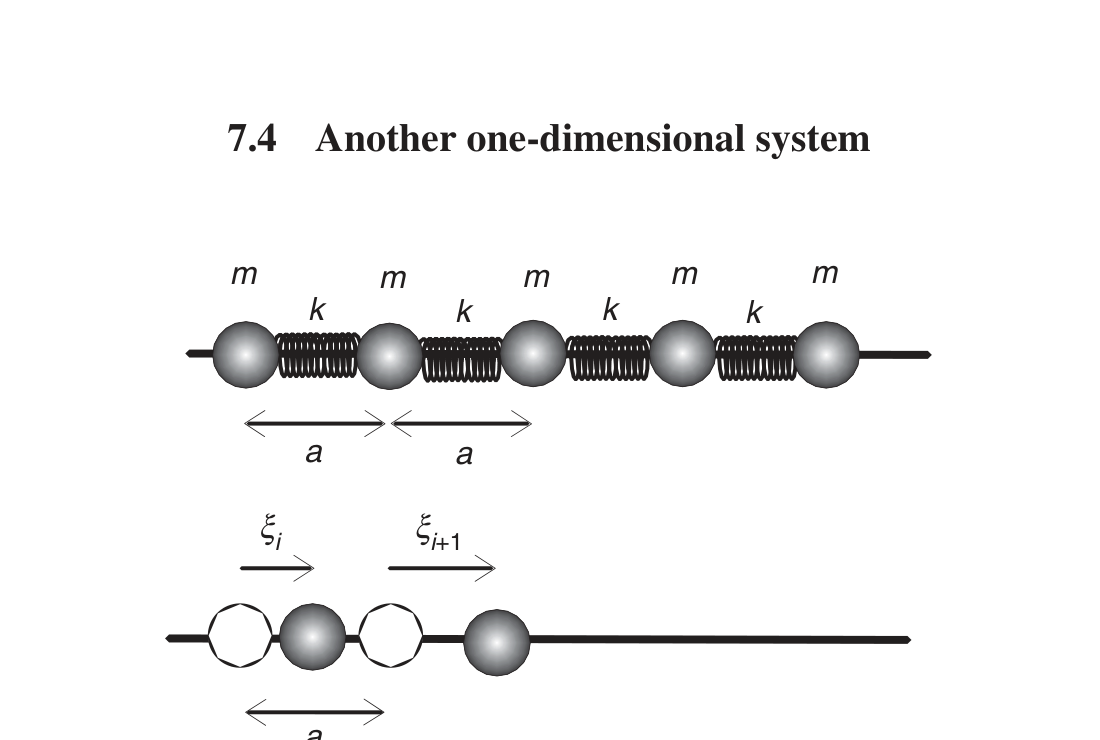
\includegraphics[width=0.55\linewidth]{../Figures/fig_7_2.png}
\caption{图 7.2　质量为 $m$ 的珠子穿在一根细而硬的金属丝上，由劲度系数为 $k$ 的弹簧相连。平衡间距为 $a$。下图显示了两颗珠子偏离平衡的距离分别为 $\xi_i$ 和 $\xi_{i+1}$。}
\end{figure}

为了更好地理解这类系统的物理，从由排成一条直线的粒子组成的一维系统入手是方便的。我们的"玩具模型"可以想象为穿在一根细而硬的金属丝上并由无质量弹簧连接起来的珠子（见图 7.2）。

设每颗珠子的质量为 $m$，每个弹簧的劲度系数为 $k$。设珠子的平衡间距为 $a$。若第 $i$ 颗珠子在平衡时的位置为 $x_i = ia$，则它偏离平衡后的位置可以表示为 $ia + \xi_i$，其中 $\xi_i$ 是第 $i$ 颗珠子偏离平衡位置的位移。粒子 $i$ 与粒子 $i+1$ 之间的距离为 $a + \xi_{i+1} - \xi_i$。弹簧的自然长度为 $a$，所以弹簧的伸长量为 $\xi_{i+1} - \xi_i$，与弹簧相关的势能为 $\frac{1}{2}k(\xi_{i+1} - \xi_i)^2$。粒子 $i$ 相对于其平衡位置（假定处于静止）的速度就是 $\dot{\xi}_i$。利用这些概念，我们可以把拉格朗日量按通常的形式写成
$$
L = T - V = \sum_i\left[\frac{m}{2}\dot{\xi}_i^2 - \frac{k}{2}(\xi_{i+1} - \xi_i)^2\right]. \eqno\hbox{(7.9)}
$$

\begin{exercise}
利用方程（7.9）给出的拉格朗日量，证明这一离散粒子系统的运动方程为
$$
m\ddot{\xi}_i - k(\xi_{i+1} - \xi_i) + k(\xi_i - \xi_{i-1}) = 0.
$$
\end{exercise}

\subsection*{7.4.1　连续杆的极限}

现在我们把这个珠子系统表示成连续系统。我们先把方程（7.9）乘以并除以 $a$，即：
$$
L = \sum_i a\left[\frac{m}{2a}\dot{\xi}_i^2 - \frac{ka}{2}\left(\frac{\xi_{i+1} - \xi_i}{a}\right)^2\right].
$$
当 $a \to 0$ 时，$m/a \to \lambda(x)$，即单位长度的质量，也就是杆在位置 $x$ 处的线质量密度。项 $(\xi_{i+1} - \xi_i)/a$ 也可以写成连续函数。令 $\xi_i = \xi(x)$，$\xi_{i+1} = \xi(x + a)$。为方便起见，我们用 $\Delta x$ 表示 $a$。于是
$$
\frac{\xi_{i+1} - \xi_i}{a} \to \frac{\xi(x + \Delta x) - \xi(x)}{\Delta x},
$$
在极限 $a \to 0$ 下，
$$
\frac{\xi_{i+1} - \xi_i}{a} \to \frac{d\xi}{dx},
$$
并且
$$
ka\left(\frac{\xi_{i+1} - \xi_i}{a}\right)^2 \to K\left(\frac{\partial\xi}{\partial x}\right)^2.
$$
求和变成对 $x$ 的积分，而
$$
L = \frac{1}{2}\int\left[\lambda(x)\left(\frac{\partial\xi}{\partial t}\right)^2 - K\left(\frac{\partial\xi}{\partial x}\right)^2\right]dx. \eqno\hbox{(7.10)}
$$

\begin{exercise}
证明 $K$ 是杨氏模量。
\end{exercise}

\begin{exercise}
证明方程（7.10）中的拉格朗日量给出波动方程。
\end{exercise}

让我们应用哈密顿原理并推导拉格朗日方程。（这一推导与我们前面关于弦的考虑类似。）根据哈密顿原理，
$$
\delta\int_{t_1}^{t_2}\int_{x_1}^{x_2}\mathcal{L}\,dx\,dt = 0,
$$
其中 $\mathcal{L} = \mathcal{L}(\xi, \dot{\xi}, \xi')$。对于手头的问题，被变分的量是 $\xi$，而不是 $x$ 或 $t$。因此，$\xi$ 在端点处的变分为零，这里端点不仅是 $t_1$ 和 $t_2$，而且还有 $x_1$ 和 $x_2$。

当我们把 $\xi$ 表示为连续变量时，它被解释为杆中一个无穷小段偏离平衡位置的位移。（这很难直观想象，所以也许在脑海中把 $\xi$ 想象为代表诸如密度之类的其他变量会有所帮助。）

为了应用变分方法，我们需要设想一个变分量 $\xi(x, t, \epsilon)$，它与"真实"量 $\xi(x, t, 0)$ 相差一个无穷小量。也就是说，我们定义
$$
\xi(x, t, \epsilon) = \xi(x, t, 0) + \epsilon\eta(x, t),
$$
其中 $\xi(x, t, 0)$ 是"真实"路径，$\epsilon$ 是一个小参数，$\eta(x, t)$ 是在端点处为零的任意函数。即
$$
\eta(x_1, t_1) = 0,
$$
以及
$$
\eta(x_2, t_2) = 0.
$$
按照通常的做法，我们写出
$$
\frac{dI}{d\epsilon} = \int_{t_1}^{t_2}dt\int_{x_1}^{x_2}dx\left[\frac{\partial\mathcal{L}}{\partial\xi}\frac{\partial\xi}{\partial\epsilon} + \frac{\partial\mathcal{L}}{\partial\dot{\xi}}\frac{\partial\dot{\xi}}{\partial\epsilon} + \frac{\partial\mathcal{L}}{\partial\xi'}\frac{\partial\xi'}{\partial\epsilon}\right] = 0.
$$
对第二项和第三项分部积分，我们得到
$$
\int_{t_1}^{t_2}\frac{\partial\mathcal{L}}{\partial\dot{\xi}}\frac{\partial\dot{\xi}}{\partial\epsilon}dt = -\int_{t_1}^{t_2}\frac{\partial}{\partial t}\left(\frac{\partial\mathcal{L}}{\partial\dot{\xi}}\right)\frac{\partial\xi}{\partial\epsilon}dt,
$$
以及
$$
\int_{x_1}^{x_2}\frac{\partial\mathcal{L}}{\partial\xi'}\frac{\partial\xi'}{\partial\epsilon}dx = -\int_{x_1}^{x_2}\frac{\partial}{\partial x}\left(\frac{\partial\mathcal{L}}{\partial\xi'}\right)\frac{\partial\xi}{\partial\epsilon}dx,
$$
从而有
$$
0 = \left.\frac{dI}{d\epsilon}\right|_{\epsilon=0} = \int_{t_1}^{t_2}dt\int_{x_1}^{x_2}dx\left[\frac{\partial\mathcal{L}}{\partial\xi} - \frac{\partial}{\partial t}\left(\frac{\partial\mathcal{L}}{\partial\dot{\xi}}\right) - \frac{\partial}{\partial x}\left(\frac{\partial\mathcal{L}}{\partial\xi'}\right)\right]\left.\frac{\partial\xi}{\partial\epsilon}\right|_{\epsilon=0}.
$$
因此，拉格朗日方程为
$$
\frac{\partial}{\partial t}\left(\frac{\partial\mathcal{L}}{\partial\dot{\xi}}\right) + \frac{\partial}{\partial x}\left(\frac{\partial\mathcal{L}}{\partial\xi'}\right) - \frac{\partial\mathcal{L}}{\partial\xi} = 0, \eqno\hbox{(7.11)}
$$
正如前面得到的（见方程（7.4））。

有趣的是，对于离散系统，每颗珠子对应一条拉格朗日方程，而对于连续系统，我们得到单独一条拉格朗日方程。另一方面，我们可以把方程（7.11）看作无穷多条方程，对应于 $x$ 的无穷多个可能的取值，每个取值对应一条方程。

\begin{exercise}
证明把方程（7.11）应用于方程（7.10）会导出波动方程。
\end{exercise}

\subsection*{推广到三维}

正如前面所指出的，我们可以容易地把上面导出的关系推广到三维。这需要把标量位移 $\xi$ 换成矢量位移 $\boldsymbol{\xi}$，其分量为 $\xi_i$，其中 $i = (1, 2, 3)$ 或 $(x, y, z)$。量 $\xi$ 表示在空间某个区域的每一点都有定义的物理量，所以它满足场的定义。事实上，我们可以让 $\xi$ 表示诸如压强、速度或电磁场等其他物理量。

场 $\xi$ 因此在每一点和每一时刻都有定义，所以 $\xi = \xi(x, y, z, t)$，拉格朗日方程为
$$
\frac{\partial}{\partial t}\left(\frac{\partial\mathcal{L}}{\partial\dot{\xi}}\right) + \frac{\partial}{\partial x}\left(\frac{\partial\mathcal{L}}{\partial(\partial\xi/\partial x)}\right) + \frac{\partial}{\partial y}\left(\frac{\partial\mathcal{L}}{\partial(\partial\xi/\partial y)}\right) + \frac{\partial}{\partial z}\left(\frac{\partial\mathcal{L}}{\partial(\partial\xi/\partial z)}\right) - \frac{\partial\mathcal{L}}{\partial\xi} = 0.
$$
该方程的第 $i$ 个分量为
$$
\frac{\partial}{\partial t}\left(\frac{\partial\mathcal{L}}{\partial(\partial\xi_i/\partial t)}\right) + \sum_{k=1}^{3}\frac{\partial}{\partial x_k}\left(\frac{\partial\mathcal{L}}{\partial(\partial\xi_i/\partial x_k)}\right) - \frac{\partial\mathcal{L}}{\partial\xi_i} = 0, \eqno\hbox{(7.12)}
$$
其中 $x_k = x, y, z$。可以注意到，$\partial/\partial t$ 和 $\partial/\partial x_k$ 有时写成全导数 $d/dt$ 和 $d/dx_k$，以表明在求导过程中还必须包含 $\xi_i$ 对 $x_k$ 或 $t$ 的隐式依赖。

使用更简单的记号可能会有所帮助，例如用 $\dot{\xi}_i$ 表示 $\partial\xi_i/\partial t$，用 $\xi'_{ik}$ 表示 $\partial\xi_i/\partial x_k$。于是方程（7.12）写成
$$
\frac{\partial}{\partial t}\left(\frac{\partial\mathcal{L}}{\partial\dot{\xi}_i}\right) + \sum_{k=1}^{3}\frac{\partial}{\partial x_k}\left(\frac{\partial\mathcal{L}}{\partial\xi'_{ik}}\right) - \frac{\partial\mathcal{L}}{\partial\xi_i} = 0. \eqno\hbox{(7.13)}
$$

\subsection*{利用泛函导数的简化记号}

我们可以利用方程（2.10）定义过的泛函导数来稍微简化记号：
$$
\frac{\delta}{\delta y} = \frac{\partial}{\partial y} - \frac{d}{dx}\frac{\partial}{\partial y'}.
$$
为了我们的目的，我们把它写成
$$
\frac{\delta\mathcal{L}}{\delta\xi_i} = \frac{\partial\mathcal{L}}{\partial\xi_i} - \sum_{k=1}^{3}\frac{d}{dx_k}\frac{\partial\mathcal{L}}{\partial\nabla\xi_i},
$$
或
$$
\frac{\delta\mathcal{L}}{\delta\xi} = \frac{\partial\mathcal{L}}{\partial\xi} - \nabla\cdot\frac{\partial\mathcal{L}}{\partial\nabla\xi}.
$$
因此，用泛函导数表示，哈密顿原理
$$
0 = \delta L = \int\left[\frac{\partial\mathcal{L}}{\partial\xi_i}\delta\xi_i - \sum_{k=1}^{3}\frac{d}{dx_k}\frac{\partial\mathcal{L}}{\partial(\partial\xi_i/\partial x_k)} + \frac{\partial\mathcal{L}}{\partial\dot{\xi}_i}\delta\dot{\xi}_i\right]d^3x
$$
可以表示为
$$
\delta L = \int\left[\frac{\delta\mathcal{L}}{\delta\xi_i}\delta\xi_i + \frac{\partial\mathcal{L}}{\partial\dot{\xi}_i}\delta\dot{\xi}_i\right]d^3x.
$$
为简单起见，并为了使上述内容更易懂，让我们回到一维系统和标量变量，把 $\xi$ 换成 $Q$。此外，让我们按通常的方式定义广义动量密度：
$$
P = \frac{\partial\mathcal{L}}{\partial\dot{Q}}.
$$
现在
$$
\mathcal{L} = \mathcal{L}(Q, \dot{Q}, Q'; x, t),
$$
所以
$$
d\mathcal{L} = \frac{\partial\mathcal{L}}{\partial Q}dQ + \frac{\partial\mathcal{L}}{\partial\dot{Q}}d\dot{Q} + \frac{\partial\mathcal{L}}{\partial Q'}dQ' + \frac{\partial\mathcal{L}}{\partial t}dt.
$$
拉格朗日方程（方程（7.11））可以写成（把 $\xi$ 换成 $Q$）
$$
\frac{\partial}{\partial t}\left(\frac{\partial\mathcal{L}}{\partial\dot{Q}}\right) + \frac{\partial}{\partial x}\left(\frac{\partial\mathcal{L}}{\partial Q'}\right) - \frac{\partial\mathcal{L}}{\partial Q} = 0.
$$
一维泛函导数可以写成
$$
\frac{\delta\mathcal{L}}{\delta Q} = \frac{\partial\mathcal{L}}{\partial Q} - \frac{\partial}{\partial x}\left(\frac{\partial\mathcal{L}}{\partial Q'}\right).
$$
类似地，
$$
\frac{\delta\mathcal{L}}{\delta\dot{Q}} = \frac{\partial\mathcal{L}}{\partial\dot{Q}} - \frac{\partial}{\partial x}\left(\frac{\partial\mathcal{L}}{\partial\dot{Q}}\right) = \frac{\partial\mathcal{L}}{\partial\dot{Q}} - \frac{\partial}{\partial x}\left(\frac{\partial\mathcal{L}}{\partial(\partial\dot{Q}/\partial x)}\right) = \frac{\partial\mathcal{L}}{\partial\dot{Q}},
$$
其中我们把 $\partial\mathcal{L}/\partial(\partial\dot{Q}/\partial x)$ 设为零，因为 $\mathcal{L}$ 不依赖于速度对位置的导数。因此，我们得到拉格朗日方程的如下形式：
$$
\frac{\partial}{\partial t}\left(\frac{\delta\mathcal{L}}{\delta\dot{Q}}\right) - \frac{\delta\mathcal{L}}{\delta Q} = 0. \eqno\hbox{(7.14)}
$$
于是我们得到了众所周知的拉格朗日方程形式，只不过我们是用泛函导数而不是偏导数来表达它。

我们还注意到，$\mathcal{L}$ 对 $\dot{P}$ 的泛函导数为
$$
\frac{\delta\mathcal{L}}{\delta\dot{P}} = \frac{\partial\mathcal{L}}{\partial\dot{P}} - \frac{\partial}{\partial x}\left(\frac{\partial\mathcal{L}}{\partial(\partial\dot{P}/\partial x)}\right).
$$
末项同样为零，所以
$$
\frac{\delta\mathcal{L}}{\delta\dot{P}} = \frac{\partial\mathcal{L}}{\partial\dot{P}},
$$
因而
$$
\frac{\delta\mathcal{L}}{\delta Q} = \frac{\partial}{\partial t}\left(\frac{\delta\mathcal{L}}{\delta\dot{Q}}\right) = \frac{\partial}{\partial t}P = \dot{P}. \eqno\hbox{(7.15)}
$$

\begin{exercise}
证明 $F(\rho) = \int c_F(\rho(r))^{5/3}\,dr$ 的泛函导数是 $\frac{5}{3}c_F(\rho(r))^{2/3}$。量 $c_F$ 是常数。
\end{exercise}

\begin{exercise}
证明 $\dfrac{\delta\mathcal{L}}{\delta\dot{\xi}} = \dfrac{\partial\mathcal{L}}{\partial\dot{\xi}}$。
\end{exercise}

\subsection*{7.4.2　连续哈密顿量与正则场方程}

对于一维系统，回忆起我们已经把连续广义动量定义为
$$
P = \frac{\partial\mathcal{L}}{\partial\dot{Q}},
$$
我们可以把哈密顿密度写成
$$
H = P\dot{Q} - \mathcal{L}.
$$
对于三维系统，我们写
$$
H = \sum_{i=1}^{3}P_i\dot{Q}_i - \mathcal{L}.
$$
因而
$$
H = \int H\,d^3x = \int\left[\sum_{i=1}^{3}P_i\dot{Q}_i - \mathcal{L}\right]d^3x.
$$
注意
$$
P_i \equiv \frac{\partial\mathcal{L}}{\partial\dot{Q}_i} = \frac{\delta\mathcal{L}}{\delta\dot{Q}_i},
$$
因为 $\mathcal{L}$ 不依赖于 $\partial\dot{Q}_i/\partial x_j$。现在坐标 $Q_i$ 和动量 $P_i$ 是独立参数 $(x, y, z, t)$ 的函数。即
$$
H = H(P_i, Q_i, \partial Q_i/\partial x_j; \mathbf{x}, t).
$$
因此
$$
dH = d\left[\int H\,d^3x\right] = \int\left[\frac{\partial H}{\partial P_i}dP_i + \frac{\partial H}{\partial Q_i}dQ_i + \sum_{k=1}^{3}\frac{\partial H}{\partial(\partial Q_i/\partial x_j)}d\left(\frac{\partial Q_i}{\partial x_k}\right) + \frac{\partial H}{\partial t}dt\right]d^3x.
$$
用泛函导数表示，这可表示为
$$
dH = \int\left[\frac{\delta H}{\delta P_i}dP_i + \frac{\delta H}{\delta Q_i}dQ_i + \frac{\partial H}{\partial t}dt\right]d^3x. \eqno\hbox{(7.16)}
$$
但回忆
$$
H = \int\left[\sum_{i=1}^{3}P_i\dot{Q}_i - \mathcal{L}\right]d^3x,
$$
所以我们可以把 $dH$ 写成
$$
dH = \int\left[P_i\,d\dot{Q}_i + \dot{Q}_i\,dP_i - \frac{\delta\mathcal{L}}{\delta Q_i}dQ_i - \frac{\delta\mathcal{L}}{\delta\dot{Q}_i}d\dot{Q}_i - \frac{\partial\mathcal{L}}{\partial t}dt\right]d^3x.
$$
根据 $P_i$ 的定义，右端第一项和第四项相消，于是剩下
$$
dH = \int\left[\dot{Q}_i\,dP_i - \frac{\delta\mathcal{L}}{\delta Q_i}dQ_i - \frac{\partial\mathcal{L}}{\partial t}dt\right]d^3x.
$$
但由方程（7.15），$\delta\mathcal{L}/\delta Q_i = \dot{P}_i$，所以
$$
dH = \int\left[-\dot{P}_i\,dQ_i + \dot{Q}_i\,dP_i - \frac{\partial\mathcal{L}}{\partial t}dt\right]d^3x. \eqno\hbox{(7.17)}
$$
令方程（7.16）和（7.17）中的对应项相等，我们得到
$$
\frac{\delta H}{\delta Q_i} = -\dot{P}_i,
$$
以及
$$
\frac{\delta H}{\delta P_i} = \dot{Q}_i,
$$
以及
$$
\frac{\partial H}{\partial t} = -\frac{\partial\mathcal{L}}{\partial t}.
$$
这些就是连续系统的哈密顿正则方程。

\begin{exercise}
证明方程（7.16）用泛函导数表达是正确的。
\end{exercise}

\begin{exercise}
证明：用普通偏导数表示时，连续系统的哈密顿正则方程失去其对称性，而具有如下形式：
$$
\frac{\partial H}{\partial Q_i} - \sum_{j=1}^{3}\frac{d}{dx_j}\frac{\partial H}{\partial(\partial Q_i/\partial x_j)} = -\dot{P}_i,
$$
$$
\frac{\partial H}{\partial P_i} = \dot{Q}_i.
$$
\end{exercise}

\section*{7.5　电磁场}

连续系统形式体系的一个有趣应用是对电磁场的处理。

回忆一下，按照定义，场是在空间某个区域的每一点都有定义的物理量。电磁场通常用麦克斯韦方程组来描述，它们是电场和磁场的散度和旋度的表达式。\footnote{亥姆霍兹定理告诉我们，如果知道了矢量场的散度和旋度，就能确定场本身。因此，场的散度和旋度常被称为场的"源"。麦克斯韦方程组就是电场和磁场的源方程。这些方程告诉我们，电磁场的源是电荷密度和电流密度。}在真空中，它们为
$$
\begin{aligned}
\nabla\cdot E &= \rho/\varepsilon_0,\\
\nabla\cdot B &= 0,\\
\nabla\times E &= -\frac{\partial B}{\partial t},\\
\nabla\times B &= \mu_0J + \varepsilon_0\mu_0\frac{\partial E}{\partial t},
\end{aligned}
\eqno\hbox{(7.18)}
$$
这里 $\rho$ 是电荷密度，$J$ 是电流密度。常数 $\varepsilon_0$ 和 $\mu_0$ 是自由空间的介电常数和磁导率，把它们放进方程是因为我们采用 SI 单位制（有时称为"合理化 MKS 单位制"）。

现在，正如从麦克斯韦方程组可以清楚地看到的那样，$E$ 和 $B$ 并不是独立的，而且，正如我们马上就要证明的，其中两条方程可以从另外两条方程推导出来。

电场 $E$ 和磁场 $B$ 可以从"势"$\phi$ 和 $A$ 得到，它们分别被称为"标量势"和"矢量势"。用势表示 $E$ 和 $B$ 的表达式为
$$
E = -\nabla\phi - \frac{\partial A}{\partial t}, \eqno\hbox{(7.19)}
$$
$$
B = \nabla\times A.
$$
如前所述，拉格朗日量是这样一种函数：它能用来生成运动方程。在这里，"运动方程"就是场方程，即麦克斯韦方程组。独立的广义坐标将是标量势 $\phi$ 和矢量势 $A$ 的分量，即 $A_x, A_y, A_z$。

能生成麦克斯韦方程组的拉格朗日密度为
$$
\mathcal{L} = \frac{1}{2}\left(\varepsilon_0E^2 - \frac{1}{\mu_0}B^2\right) - \rho\phi + J\cdot A, \eqno\hbox{(7.20)}
$$
其中 $E^2$ 和 $B^2$ 要用势来表示，即利用方程（7.19）。注意，这个拉格朗日密度由以下部分组成：（1）电磁场中的能量密度，（2）电荷密度 $\rho$ 与标量势 $\phi$ 相互作用产生的能量，以及（3）电流密度 $J$ 与矢量势 $A$ 的相互作用。为了确定场方程，我们使用如下形式的拉格朗日方程：
$$
\frac{d}{dt}\frac{\partial\mathcal{L}}{\partial\dot{Q}_i} + \sum_{j=1}^{3}\frac{d}{dx_j}\frac{\partial\mathcal{L}}{\partial(\partial Q_i/\partial x_j)} - \frac{\partial\mathcal{L}}{\partial Q_i} = 0,
$$
其中 $Q_i$ 是 $\phi$ 或 $A$ 的三个分量之一。我们现在证明，对这一拉格朗日方程求值会导出麦克斯韦方程组。让我们先把 $Q_i$ 取为 $\phi$，因为这是最简单的情形。拉格朗日方程变为
$$
\frac{d}{dt}\frac{\partial\mathcal{L}}{\partial\dot{\phi}} + \sum_{j=1}^{3}\frac{d}{dx_j}\frac{\partial\mathcal{L}}{\partial(\partial\phi/\partial x_j)} - \frac{\partial\mathcal{L}}{\partial\phi} = 0. \eqno\hbox{(7.21)}
$$
由方程（7.20）和（7.19）我们看出，拉格朗日密度不依赖于 $\dot{\phi}$。但它确实通过 $E$ 对 $\partial A/\partial t$ 的依赖而依赖于 $\dot{A}_i$。它还通过 $\nabla\phi$ 和 $\nabla\times A$ 依赖于 $\phi$ 和 $A$ 的空间导数。

尽管如此，$\partial\mathcal{L}/\partial\dot{\phi} = 0$，所以我们可以舍去方程（7.21）中的第一项。第二项为
$$
T_2 = \frac{d}{dx}\frac{\partial\mathcal{L}}{\partial(\partial\phi/\partial x)} + \frac{d}{dy}\frac{\partial\mathcal{L}}{\partial(\partial\phi/\partial y)} + \frac{d}{dz}\frac{\partial\mathcal{L}}{\partial(\partial\phi/\partial z)}.
$$
$B$ 不依赖于 $\phi$，而 $E$ 按照
$$
E = -\nabla\phi = -\left(\hat{x}\frac{\partial\phi}{\partial x} + \hat{y}\frac{\partial\phi}{\partial y} + \hat{z}\frac{\partial\phi}{\partial z}\right)
$$
依赖于 $\phi$ 的空间导数，所以
$$
\frac{\partial\mathcal{L}}{\partial(\partial\phi/\partial x)} = -\frac{\partial\mathcal{L}}{\partial E_x}, \qquad
\frac{\partial\mathcal{L}}{\partial(\partial\phi/\partial y)} = -\frac{\partial\mathcal{L}}{\partial E_y}, \qquad
\frac{\partial\mathcal{L}}{\partial(\partial\phi/\partial z)} = -\frac{\partial\mathcal{L}}{\partial E_z}.
$$
因此
$$
T_2 = -\frac{d}{dx}\frac{\partial\mathcal{L}}{\partial E_x} - \frac{d}{dy}\frac{\partial\mathcal{L}}{\partial E_y} - \frac{d}{dz}\frac{\partial\mathcal{L}}{\partial E_z} = -\nabla\cdot\left(\frac{\partial\mathcal{L}}{\partial E_x}\hat{x} + \frac{\partial\mathcal{L}}{\partial E_y}\hat{y} + \frac{\partial\mathcal{L}}{\partial E_z}\hat{z}\right) = -\varepsilon_0\nabla\cdot E,
$$
因为
$$
\frac{\partial\mathcal{L}}{\partial E_x} = \frac{\partial\left(\frac{1}{2}\varepsilon_0E^2\right)}{\partial E_x} = \frac{\partial\left[\frac{1}{2}\varepsilon_0\left(E_x^2 + E_y^2 + E_z^2\right)\right]}{\partial E_x} = \varepsilon_0E_x.
$$
最后，第三项为
$$
T_3 = -\frac{\partial\mathcal{L}}{\partial\phi} = +\rho.
$$
因而
$$
T_1 + T_2 + T_3 = 0 - \varepsilon_0\nabla\cdot E + \rho = 0,
$$
所以
$$
\nabla\cdot E = \rho/\varepsilon_0.
$$
这样我们就推导出了第一条麦克斯韦方程。

另一条麦克斯韦方程如下获得。令连续广义坐标为 $A_x$，即矢量势的 $x$ 分量。注意
$$
E = -\nabla\phi - \frac{\partial A}{\partial t}.
$$
因此
$$
E = E_x\hat{x} + E_y\hat{y} + E_z\hat{z} = \left(-\frac{\partial\phi}{\partial x} - \dot{A}_x\right)\hat{x} + \left(-\frac{\partial\phi}{\partial y} - \dot{A}_y\right)\hat{y} + \left(-\frac{\partial\phi}{\partial z} - \dot{A}_z\right)\hat{z}.
$$
类似地，$B = \nabla\times A$，因此
$$
B = (A'_{zy} - A'_{yz})\hat{x} + (A'_{xz} - A'_{zx})\hat{y} + (A'_{yx} - A'_{xy})\hat{z}.
$$
拉格朗日方程为
$$
\frac{d}{dt}\frac{\partial\mathcal{L}}{\partial\dot{A}_x} + \sum_{j=1}^{3}\frac{d}{dx_j}\frac{\partial\mathcal{L}}{\partial A'_{xj}} - \frac{\partial\mathcal{L}}{\partial A_x} = 0.
$$
由于 $\mathcal{L}$ 中唯一依赖于 $\dot{A}_x$ 的项是 $\varepsilon_0E^2/2$，唯一依赖于 $A'$ 的项是 $-B^2/2\mu_0$，而唯一依赖于 $A_x$ 的项是 $J\cdot A$，让我们写出
$$
0 = \frac{d}{dt}\frac{\partial(\varepsilon_0E^2/2)}{\partial\dot{A}_x} + \sum_{j=1}^{3}\frac{d}{dx_j}\frac{\partial(-B^2/2\mu_0)}{\partial A'_{xj}} - \frac{\partial(J\cdot A)}{\partial A_x},
$$
$$
= \frac{d}{dt}\left[\frac{\varepsilon_0}{2}\frac{\partial E^2}{\partial E}\frac{\partial E}{\partial\dot{A}_x}\right] - \sum_{j=1}^{3}\frac{d}{dx_j}\left[\frac{1}{2\mu_0}\frac{\partial B^2}{\partial B}\frac{\partial B}{\partial A'_{xj}}\right] - \frac{\partial}{\partial A_x}\left(J_xA_x + J_yA_y + J_zA_z\right),
$$
$$
= -\varepsilon_0\frac{dE_x}{dt} + \frac{1}{\mu_0}\left(\frac{\partial B_z}{\partial y} - \frac{\partial B_y}{\partial z}\right) - J_x,
$$
$$
= -\varepsilon_0\frac{dE_x}{dt} + \frac{1}{\mu_0}(\nabla\times B)_x - J_x,
$$
或
$$
(\nabla\times B)_x = \varepsilon_0\mu_0\frac{\partial E_x}{\partial t} + \mu_0J_x.
$$
类似地，$A$ 的另外两个分量导出方程（7.18）中最后一条麦克斯韦方程的另外两个分量。

于是我们看到，拉格朗日量的连续形式体系导出了两条麦克斯韦方程。但另外两条麦克斯韦方程呢？它们可以从我们推导出的两条方程得到。具体地说，由于 $B = \nabla\times A$，于是
$$
\nabla\cdot B = \mathrm{div}(B) = \mathrm{div}(\nabla\times A) = \mathrm{div}\,\mathrm{curl}(A) = 0,
$$
因为任何矢量函数的旋度的散度都为零。类似地，由于 $E = -\nabla\phi - \partial A/\partial t$，
$$
\nabla\times E = \mathrm{curl}(E) = -\mathrm{curl}\,\mathrm{grad}\,\phi - \frac{\partial}{\partial t}(\mathrm{curl}\,A) = -\frac{\partial B}{\partial t},
$$
因为任何标量函数的梯度的旋度都为零。

我们这种对电磁场的描述存在一个困难，那就是电磁场能量中没有任何一项与动能等价，所以我们无法定义广义动量，也无法定义哈密顿密度。

\section*{7.6　结论}

在这短短的一章中，我们展示了用拉格朗日方法处理连续系统的步骤。我希望你已经认识到，在我们这一发展过程中主要的困难是繁琐的记号。如果你能越过那些看起来复杂的方程，你就会认识到，其本质概念与我们用于离散系统的概念并没有什么不同。

我们不仅得到了连续场的拉格朗日方程，还发展了哈密顿量和哈密顿正则运动方程。最后，我们看到了拉格朗日密度 $\mathcal{L}$ 描述电磁场。

本章概述的理论还可以应用于其他几个领域，如流体动力学，并且在量子场论的发展中尤为重要。

\section*{7.7　习题}

7.1　证明：在一维拉格朗日密度上加上 $\dfrac{\partial L}{\partial t} + \dfrac{\partial L}{\partial x}$ 不会改变拉格朗日方程。

7.2　考虑拉格朗日密度
$$
\mathcal{L} = \frac{i\hbar}{2}(\psi^*\dot{\psi} - \dot{\psi}^*\psi) - \frac{\hbar^2}{2m}\nabla\psi^*\cdot\nabla\psi - V(r)\psi^*\psi.
$$
证明 $\dfrac{\delta\mathcal{L}}{\delta\psi^*}$ 生成薛定谔方程。

7.3　考虑拉格朗日密度
$$
\mathcal{L} = \frac{\lambda}{2}\left(\frac{\partial\eta}{\partial t}\right)^2 - \frac{1}{2}v^2\left(\frac{\partial\eta}{\partial x}\right)^2 - \frac{1}{2}\mu^2\eta^2,
$$
其中 $\lambda$ 是线质量密度，$v$ 是波速，$\mu^2$ 是常数。证明拉格朗日方程生成一维克莱因-戈登方程：
$$
\frac{\partial^2\eta}{\partial t^2} - \frac{v^2}{\lambda}\frac{\partial^2\eta}{\partial x^2} + \frac{\mu^2}{\lambda}\eta = 0.
$$

7.4　无旋等熵流体流动的拉格朗日密度为
$$
\mathcal{L} = \rho\frac{\partial\phi}{\partial t} - \frac{1}{2}\rho(\nabla\phi)^2 - \rho U - \rho\varepsilon(\rho),
$$
其中 $\phi$ 是速度势（$v = -\nabla\phi$），$\rho$ 是密度，$\varepsilon$ 是内能密度，$U$ 是单位质量的势能。拉格朗日密度是 $\phi$ 和 $\rho$ 的函数，它们可以看作广义场。（a）证明广义动量密度是 $\rho$。（b）证明广义动量密度的运动方程就是流体的连续性方程。

7.5　"声场"由气体中的纵向振动构成。若气体元的位移由 $\eta$ 描述（其分量为 $\eta_i = \eta_x, \eta_y, \eta_z$），则动能密度为
$$
T = \frac{1}{2}\rho_0(\dot{\eta}_x^2 + \dot{\eta}_y^2 + \dot{\eta}_z^2),
$$
其中 $\rho_0$ 是质量密度的平衡值。势能密度为
$$
V = -P_0\nabla\cdot\eta + \frac{1}{2}\gamma P_0(\nabla\cdot\eta)^2,
$$
其中 $P_0$ 是压强的平衡值，$\gamma$ 是定压比热与定容比热之比。（a）写出拉格朗日密度。（b）得到运动方程。（c）解释为什么 $P_0\nabla\cdot\eta$ 这一项对运动方程没有贡献。（d）合并运动方程，得到一个三维波动方程。

7.6　考虑一个可以表示成密度函数 $F$ 的函数 $F = F(q_i, p_i)$，使得 $F = \int F\,d^3x$。假定 $F$ 不显式地依赖于时间。（a）证明 $F$ 的时间导数可以表示为
$$
\frac{dF}{dt} = \int\left[\frac{\delta F}{\delta Q_i}\dot{Q}_i + \frac{\delta F}{\delta P_i}\dot{P}_i\right]d^3x.
$$
（b）应用正则方程，得到泊松括号的类似物。
